\documentclass[12pt,a4paper]{report}
\usepackage[utf8]{inputenc}
\usepackage[T1]{fontenc}
\usepackage[english,italian]{babel}
\usepackage{amsmath}
\usepackage{amssymb}
\usepackage{amsfonts}
\usepackage{mathrsfs}
\usepackage{graphicx}
\usepackage{amsthm}
\usepackage{newlfont}
\usepackage{color}
\usepackage{natbib}
\usepackage{float}
\usepackage{textcomp}

\textwidth=450pt\oddsidemargin=0pt

\begin{document}

\begin{titlepage}

%
%
% UNA VOLTA FATTE LE DOVUTE MODIFICHE SOSTITUIRE "RED" CON "BLACK" NEI COMANDI \textcolor
%
%
\begin{center}
{{\Large{\textsc{Alma Mater Studiorum $\cdot$ Universit\`a di Bologna}}}} 
\rule[0.1cm]{15.8cm}{0.1mm}
\rule[0.5cm]{15.8cm}{0.6mm}
\\\vspace{3mm}

{\small{\bf Scuola di Scienze \\ 
Dipartimento di Fisica e Astronomia\\
Corso di Laurea in Fisica}}

\end{center}

\vspace{23mm}

\begin{center}\textcolor{black}{
%
% INSERIRE IL TITOLO DELLA TESI
%
{\LARGE{\bf Analisi della complessità di reti neurali generate tramite algoritmi genetici}}\\
}\end{center}

\vspace{50mm} \par \noindent

\begin{minipage}[t]{0.47\textwidth}
%
% INSERIRE IL NOME DEL RELATORE CON IL RELATIVO TITOLO DI DOTTORE O PROFESSORE
%
{\large{\bf Relatore: \vspace{2mm}\\\textcolor{black}{
Dott. Enrico Giampieri}\\\\
%
% INSERIRE IL NOME DEL CORRELATORE CON IL RELATIVO TITOLO DI DOTTORE O PROFESSORE
%
% SE NON AVETE UN CORRELATORE CANCELLATE LE PROSSIME 3 RIGHE
%
\textcolor{black}{
\bf Correlatore: 
\vspace{2mm}\\
Dott. Nico Curti\\\\}}}
\end{minipage}
%
\hfill
%
\begin{minipage}[t]{0.47\textwidth}\raggedleft \textcolor{black}{
{\large{\bf Presentata da:
\vspace{2mm}\\
%
% INSERIRE IL NOME DEL CANDIDATO
%
Mattia Ceccarelli}}}
\end{minipage}

\vspace{38mm} %qui sarebbe stato 40mm

\begin{center}
%
% INSERIRE L'ANNO ACCADEMICO
%
Anno Accademico \textcolor{black}{ 2017/2018}
\end{center}

\end{titlepage}
 
\small\tableofcontents
%\clearpage{\pagestyle{empty}\cleardoublepage}

\newpage

\vspace*{125px}
\LARGE\textit{Abstract}
\normalsize

L'enorme quantità di dati sviluppata tramite le infrastrutture moderne richiede strumentazioni di analisi sempre più precise, rapide e performanti. 
Per questo negli ultimi anni i metodi del machine learning hanno visto un'esplosione nella ricerca e nell'utilizzo di algoritmi mano a mano più efficienti per ogni disciplina. 
Due tra le numerose famiglie di tecniche appartenenti alla sfera del machine learning sono reti neurali e algoritmi genetici. 
Il progetto di tesi presentato ha come obiettivo quello di verificare la possibilità di evolvere la struttura di una rete neurale attraverso un algoritmo genetico in modo da automatizzarne il processo di costruzione, che ad oggi consiste in un procedimento di trial and error.
La simulazione programmata consiste nell'evoluzione di una popolazione iniziale randomica di neural network tramite le tipiche metodologie di un algoritmo genetico, adattate al caso particolare di una funzione senza un predeterminato numero di variabili, il quale diventa un parametro della ricerca. 
Le reti verranno addestrate e valutate nella separazione di due classi di punti in dataset artificiali per verificare la bontà dell'algoritmo. 
Dopodiché lo studio si concentrerà sull'analisi del come e quando la rumorosità dei dati influenzi la complessità della rete ottenuta dall'algoritmo genetico, la quale viene misurata attraverso specifiche caratteristiche.
La classificazione nei dataset testati è buona utilizzando un classico controllo binario del successo nella risposta della rete (giusto/sbagliato) tuttavia è migliore utilizzando un particolare metro di valutazione chiamato logarithmic loss.  
Lo studio sulla complessità della rete mostra una rilevante dipendenza di questa dalla rumorosità del dataset; inoltre, risulta che la separazione tra train test e test set nell'addestramento è sufficiente a regolarizzare la complessità della rete senza altri tipi di penalizzazione.

\newpage
\normalsize 

\chapter{Introduzione}

Il progetto di tesi presentato ha come obiettivo verificare la possibilità di evolvere la struttura di una rete neurale attraverso un algoritmo genetico in modo da automatizzarne il processo di costruzione, che ad oggi consiste in un procedimento di "\textit{trial and error}".
Le reti verranno valutate nella separazione di due classi di punti in dataset artificiali semplici per verificare la bontà dell'algoritmo. 
Dopodiché lo studio si concentrerà sull'analisi del come e quando la rumorosità dei dati influenzi la complessità della rete ottenuta dall'algoritmo genetico.

In questo capitolo verranno presentati i principali concetti teorici essenziali alla comprensione delle Metodologie applicate, tra i quali naturalmente la base di un algoritmo genetico e di rete neurale.

Il secondo capitolo include la spiegazione di come questi concetti siano stati adattati nel caso presentato ed in particolare come vengano implementati algoritmi genetici e reti neurali, cosa si intenda per "individuo" e "popolazione", quali dataset siano stati utilizzati e come venga effettuata la presa e l'analisi dati.

Nel terzo capitolo vengono presentati i risultati separati in una parte di valutazione della capacità di classificazione dell'algoritmo e nella seconda parte, in cui vengono mostrati i risultati relativi alla struttura della rete in funzione della rumorosità dei dataset. 

Infine vengono tratte le relative conclusioni e vengono proposti sviluppi futuri sull'algoritmo.

\section{Algoritmi Genetici}\label{alg-gen} 

Gli algoritmi genetici sono software di ricerca ispirati dalla selezione naturale applicata ad una popolazione di individui, i quali vengono valutati nello svolgimento di un \textit{task} (Ambiente).
Il parametro che differenzia soluzioni migliori o peggiori è il \textit{fitness}, misurato attraverso la \textit{funzione di fitness} la quale dipende dal problema.
L' evoluzione della popolazione avviene attraverso la selezione dei migliori individui che passeranno il loro \textit{cromosoma} alla generazione successiva.

Sono stati inventati da John Holland negli anni '60 e sono stati sviluppati dallo stesso Holland e dai suoi studenti e colleghi tra gli anni '60 e '70 \cite{genetic-algorithm-mitchell}.
L'idea iniziale non era quella di risolvere un particolare problema, in contrasto con l'approccio adottato dai ricercatori per algoritmi evolutivi e programmazione evolutiva, ma di studiare l'adattamento naturale delle specie e trovare un modo per importare questo meccanismo in un computer.

Nel suo libro "\textit{Adaptation in Natural and Artificial Systems}" Holland presenta gli algoritmi genetici come un'astrazione dell'evoluzione biologica: gli algoritmi genetici sono un metodo per muovere una popolazione di \textit{cromosomi} ad una nuova popolazione usando una specie di Selezione Naturale insieme ad operatori ispirati dalla biologia.
         
\subsection{Operatori}

I principali operatori che compongo un semplice algoritmo genetico sono\cite{genetic-algorithm-mitchell}:

\paragraph{Selezione} Questo operatore seleziona i migliori individui, più è alto è il fitness e più è probabile che un individuo venga scelto per creare la nuova generazione

\paragraph{Crossover} L'operatore di Crossover produce un taglio nel genoma degli individui ``genitori`` per formare due individui ''figli'': per esempio prendendo le due stringhe 111000 e 000111, producendo un taglio alla terza posizione otterremo le stringhe  111111 e 000000.

\paragraph{Mutazione} L'operatore di mutazione si occupa di cambiare casualmente uno o più caratteri di individui scelti a caso nella popolazione.

Il funzionamento di un tipico algoritmo genetico,come descritto da \cite{genetic-algorithm-mitchell} una volta definito il problema,  procede in questo modo:

\subsection{Struttura di un Algoritmo Genetico}

\begin{enumerate}
 \item Creazione casuale di \textit{n} elementi, che rappresentano la prima popolazione. 
 \item Calcolo del fitness $f(x)$ di ogni soluzione $x$ della popolazione.
 \item Fino a che non sono stati generati \textit{n} discendenti ripetere:
 \begin{enumerate}
  \item[a.] Selezione di due genitori dalla popolazione dove un individuo può anche essere scelto più volte.
  \item[b.] Con probabilità $p_{c}$ (probabilità di crossover) applicare l'operatore di crossover sui due genitori. Nel caso non avvenisse alcun crossover, copiare i genitori.
  \item[c.] Con probabilità $p_{m}$ (probabilità di mutazione) applicare l'operatore di mutazione sui figli.
 \end{enumerate}
 \item Sostituire la vecchia popolazione con la nuova generazione e ripetere dal secondo passaggio.
\end{enumerate}

Ogni iterazione di questo processo è chiamata \textit{generazione}.

Il classico esempio di utilizzo di un algoritmo genetico è la ricerca dei massimi di una funzione.
In tal caso, un individuo è rappresentato da una stringa di bit, la \textit{funzione di fitness} è la funzione stessa e il \textit{fitness} delle soluzioni è il valore della funzione calcolato nel punto di cui l'individuo è la rappresentazione binaria.
Oltre ad essere l'esempio più semplice risulta anche quello più significativo: di fatto lo scopo di un algoritmo genetico è l'ottimizzazione.  

Ad oggi gli algoritmi genetici vengono utilizzati in molti campi per l'ottimizzazione di funzioni arbitrarie non necessariamente continue o derivabili.

\section{Reti Neurali}

Una rete neurale è una struttura interconnessa di semplici unità procedurali, chiamate nodi. La loro funzionalità si ispira ai neuroni del regno animale. La capacità di elaborazione della rete neurale è contenuta nella ``forza`` delle connessioni tra nodi, espressa dai \textit{pesi} dei collegamenti, ottenuti da processi di \textit{ addestramento} o \textit{apprendimento}. \cite{neural-net-gurney}

L'idea di rete neurale proviene dalle ricerche sull'apprendimento di D.O. Hebb degli anni '40, citando dal suo libro \textit{"Organization of Behavior"} \cite{hebb-learning}:

\begin{quote}
 \begin{center}
  \textit{Let us assume that the persistence or repetition of a reverberatory activity (or "trace") tends to induce lasting cellular changes that add to its stability.[…] When an axon of cell A is near enough to excite a cell B and repeatedly or persistently takes part in firing it, some growth process or metabolic change takes place in one or both cells such that A's efficiency, as one of the cells firing B, is increased}
 \end{center}
\end{quote} 

Che è la spiegazione della plasticità neuronale (per \textit{firing} si intende l'invio di un segnale, elettrico in questo caso).
Dalla cosiddetta "\textit{Hebbian Theory}" deriva il modello computazionale di rete neurale di  Warren McCulloch e Walter Pitts chiamato "\textit{Threshold logic}" che aprì la ricerca sulle reti neurali e portò in seguito al "\textit{Perceptron}", trattato nella sezione \ref{percettrone}, o al più moderno \textit{deep learning},  oggi applicato in moltissimi campi come il riconoscimento di file audio, la bioinformatica, il riconoscimento di immagini e perfino i giochi da tavolo.

\subsection{Perceptron}\label{percettrone}

Il \textit{perceptron} è stato sviluppato negli anni '50 e '60 dal ricercatore Frank Rosenblatt ispirandosi ai lavori antecedenti di Warren McCulloch e Walter Pitts \cite{neural-net-nielsen}.
È l'unità di base di una rete neurale e il suo funzionamento è il seguente:
il \textit{perceptron} riceve $n$ valori in ingresso $x_{1},x_{2},...,x_{n}$ e restituisce $1$ o $0$ a seconda che la somma pesata degli input superi o no un valore di soglia, con pesi $w_{1},w_{2},...,w_{n}$.
Ad esempio nel \textit{perceptron} mostrato in figura \ref{perceptron}:

\begin{figure}[H]
 \centering
 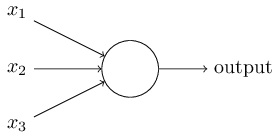
\includegraphics[scale = 0.7]{images/perceptron.png}
 \caption{\textit{Perceptron con 3 input ed un output}}
 \label{perceptron}
\end{figure}

l'output sarà determinato da:

\begin{center}
$\begin{cases}
 0 \text{ se } \sum_{i} x_{i}w_{i} \leq valore\text{ }di\text{ }soglia\\
 1 \text{ se } \sum_{i} x_{i}w_{i} > valore\text{ }di\text{ }soglia 
\end{cases} $
\end{center}

anche se è più comune trovare la scrittura:

\begin{center}
$\begin{cases}
 0 \text{ se } \sum_{i} x_{i}w_{i} + b \leq 0\\
 1 \text{ se } \sum_{i} x_{i}w_{i} + b > 0
\end{cases}$
\end{center}

dove $b$ è detto \textit{bias} del perceptron.
È attraverso \textit{pesi} e \textit{bias} che il perceptron può soppesare diverse prove e compiere decisioni.

Tuttavia se la rete contenesse perceptron, anche un piccolo cambiamento nei parametri interni potrebbe causare un cambiamento netto nel comportamento della rete [\cite{neural-net-nielsen}], per questo è preferibile utilizzare una \textit{funzione di attivazione} che rende continuo l'output di un nodo.
Un esempio di funzione di attivazione è la sigmoide definita come:

\begin{equation} \label{sigma}
 \sigma(z) = \frac{1}{1+e^{-z}} 
\end{equation}

e l'output di un nodo della rete diventa :

\begin{equation} \label{z}
  y = \sigma(\sum_{i}{x_{i}w_{i}} + b)
\end{equation}

risultato che è continuo e compreso tra zero ed uno.

Un altro tipo di funzione di attivazione è la \textit{Rectified Linear Units} o \textit{ReLU} e si presenta come:

\begin{equation}
 y(x) = max \{0,x\} 
\end{equation}

La \textit{ReLU} viene spesso usata per risolvere il problema del \textit{vanishing gradient} nel deep learning: quando la funzione sigmoidale è molto vicina ad 1 la derivata si annulla per problemi numerici e ciò rende difficile il tuning dei pesi dei primi layer. Il problema risulta più grave per reti molto profonde.

\begin{figure}[H]
 \centering
 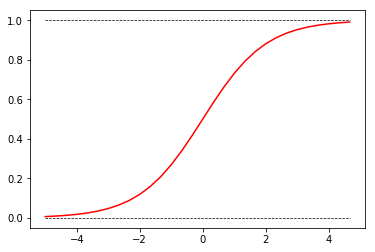
\includegraphics[scale = 0.5]{images/sigmoide.png}
 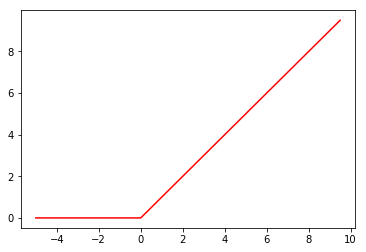
\includegraphics[scale = 0.5]{images/relu.png}
 \caption{\textit{confronto tra due funzioni di attivazione: a sinistra sigmoidale e a destra ReLU}}
 \label{sigmarelu}
\end{figure}

La scelta della migliore funzione di attivazione non è univoca e dipende dal problema che viene affrontato.

\newpage

\subsection{Struttura \textit{fully connected}}

La struttura di una rete neurale \textit{fully connected} composta da molti \textit{layer} di neuroni è come quella mostrata in figura \ref{net}:

\begin{figure}[H]
 \centering
 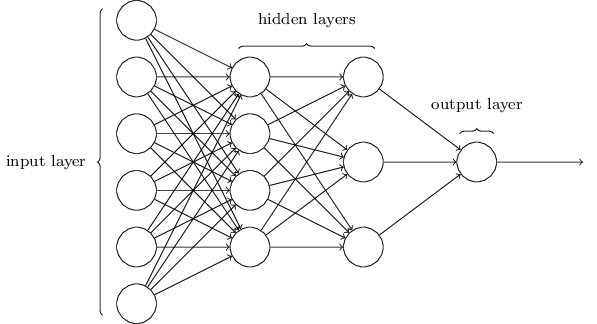
\includegraphics[scale = 0.5]{images/net.png}
 \caption{\textit{Esempio di rete neurale fully connected in cui viene mostrata la distinzione tra input layer, hidden layer e output layer}}
 \label{net}
\end{figure} 

In una rete come questa ad ogni collegamento è associato un peso e ad ogni nodo è associato un \textit{bias}: gli output dei \textit{neuroni} del \textit{layer} di input diventano a loro volta valori in ingresso del \textit{layer} successivo in un procedimento a catena fino all'ultimo \textit{layer}, che restituisce la risposta della rete. 
Le reti \textit{fully connected} sono considerate \textit{universal approximators}, nel senso che dati abbastanza parametri sono in grado di approssimare qualsiasi funzione per quanto complessa.\cite{neural-net-nielsen}

L'addestramento della rete consiste nel valutarne gli output in un determinato set di dati, chiamato \textit{training dataset}, confrontarli con i valori attesi, forniti dallo stesso \textit{dataset}, e modificare pesi e \textit{bias} in modo che la risposta si avvicini a ciò che ci si aspetta.

L'algoritmo di addestramento più utilizzato è la \textit{Backpropagation}, che è la modalità utilizzata per i \textit{Multy Layer Perceptron} in questa prova.

L'idea su cui si basa è di valutare l'errore commesso da ogni output della rete, dopo un' inizializzazione casuale dei pesi, in base all'output atteso e di retro propagare lungo la rete gli scarti per aggiornare il valore dei pesi \cite{backprop}.
Indicando con:

\begin{enumerate}
 \item[-] $t_{k}$: risultato atteso al $k$-esimo output;
 \item[-] $y_{k}$: risultato ottenuto al $k$-esimo output;
 \item[-] $w$: peso generico;
 \item[-] $W$: l'insieme dei pesi.
\end{enumerate}

L'errore commesso dal $k$-esimo output è stimato da:

\begin{equation}
 \centering
 E_{k} = (t_{k}-y_{k})
\end{equation}

Da cui possiamo definire la funzione d'errore come:

\begin{equation}
 \centering
 J(W) = \sum_{k = 1}^{N}\frac{1}{2}E_{k}^2 = \sum_{k = 1}^{N}\frac{1}{2}(t_{k}-y{k})^2
\end{equation}

Si procede poi nel correggere i pesi partendo dall'output fino all'input nel modo seguente:

\begin{equation}
 \centering
 w = w + \delta w = w + \eta \frac{\partial J}{\partial w}
\end{equation}

dove $\eta$ è una costante che garantisce un'opportuna convergenza ai pesi. 
Lo scopo è quello di trovare un minimo alla funzione d' errore. \cite{backprop}

\chapter{Metodologia}

In questo capitolo verranno descritti i metodi utilizzati per l'ottimizzazione di una rete neurale \textit{fully connected} attraverso un algoritmo genetico: l' obiettivo è quello di evolvere la struttura degli \textit{hidden layer} della rete al fine di classificare al meglio un dataset separato in due classi di dati.

\section{Popolazione di reti neurali}

L'algoritmo genera la prima popolazione di oggetti \textit{Random Network} casualmente, i parametri interni sono stati scelti in modo che questa fosse limitata e non raggiungesse subito un risultato ottimale.
In particolare il numero di layer è compreso tra 1 e 5 mentre il numero massimo di neuroni per layer è 25.
La popolazione è stata mantenuta al massimo di 20 individui per lo stesso motivo.
Il \textit{cromosoma} di un individuo è quindi una lista di numeri di lunghezza variabile e l'algoritmo genetico è stato adattato a questo problema: la ricerca di un minimo in uno spazio in cui il numero di variabili non è definito.

\section{Operatori}

La differenza nell'utilizzare cromosomi di lunghezza variabile si ritrova soprattutto negli operatori dell'algoritmo genetico scritto \textit{ad hoc} per il progetto che devono gestire una variabile che normalmente non rappresenterebbe un problema. 
Per questo ogni operatore è stato adattato per fare in modo che sia possibile esplorare lo spazio delle soluzioni anche in tal senso.

\subsection{Crossover}

Il Crossover si differenzia da quello di un algoritmo genetico in cui la lunghezza di ogni cromosoma sia prestabilita. 
Infatti, è facile che i due genitori selezionati non abbiano lo stesso numero di hidden layer: in questo caso non è possibile "tagliare" il cromosoma nello stesso punto (come mostrato nel capitolo \ref{alg-gen}).
Inoltre è necessario che la lunghezza dei figli possa essere diversa da quella dei genitori in modo da non limitare le possibilità di esplorazione.

Seguendo questi propositi, vengono scelti casualmente due punti di taglio, uno per genitore, dalla mediana di tre interi casuali (questo per fare in modo che la lunghezza non cambi troppo tra una generazione e la successiva, come mostrato in figura \ref{median}).
Dopodiché il crossover procede come in un classico algoritmo genetico, ossia restituendo due figli, combinazione delle parti tagliate.

\begin{figure}[H]
 \centering
 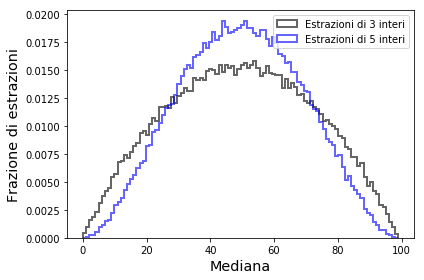
\includegraphics[scale = 0.7]{images/median-3-5}
 %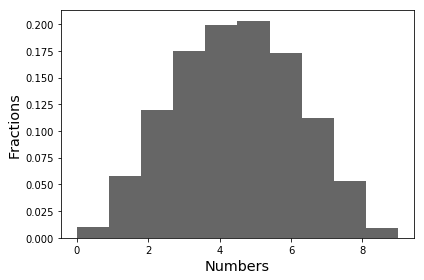
\includegraphics[scale = 0.5]{images/median-5}
 \caption{\textit{In figura viene mostrato il risultato di 100000 estrazioni di serie da 3(in nero) e 5(in blu) interi casuali (da 1 a 100) dalle quali viene estratta la mediana. Aumentando il numero di numeri casuali da cui estrarre la mediana, il picco si stringe e si alza al centro. In viola un'estrazione uniforme.}}
 \label{median}
\end{figure}

Un esempio di funzionamento, scelti i genitori:

\begin{center}
 genitore 1 = [10,3,4,11];  genitore 2 = [7,23,1,2,19]\\
\end{center}

e prendendo due tagli rispettivamente alla $3^{a}$ e $2^{a}$ posizione si ottengono:

\begin{center}
 figlio 1 = [10,3,4,1,2,19]; figlio 2 = [7,23,11]
\end{center}

i quali popoleranno la generazione successiva.

\subsection{Mutazione}

Anche il processo di mutazione ha subito qualche variazione, infatti, occorre che anche la lunghezza del cromosoma possa cambiare a seguito dell'azione di questo operatore.
Per fare ciò sono state introdotte due probabilità indipendenti: $p_{m} = 5$\textdiscount \text{ }rappresenta la probabilità che un layer qualsiasi del cromosoma venga modificato aggiungendo o togliendo un neurone, $p_{l} = 5$\textdiscount \text{ }rappresenta invece la probabilità che venga aggiunto o rimosso un layer dalla rete.

\subsection{Selezione}

Nella varietà di operatori di selezione, verranno comparati i risultati di due algoritmi, scelti per la semplicità di implementazione che nulla toglie alla capacità di questi di evolvere il sistema.

\begin{enumerate}
 \item Il primo, denominato \textit{random mate}, è il più rapido: partendo da una popolazione ordinata per miglior \textit{fitness} passa alla nuova generazione un' \textit{élite} di individui pari al 20\textdiscount.
 Poi scorre dall'inizio la popolazione per il primo genitore, mentre il secondo genitore viene scelto a caso. 
 Questo avviene fino a che la generazione successiva non è riempita.
 
 \item Il secondo, denominato \textit{all sons}, è concettualmente più semplice ma richiede molto più tempo per completare una run: continuando a mantenere un 20\textdiscount di \textit{élite}, in una popolazione viene fatto il crossover di ogni coppia possibile di individui.
 Di questi vengono scelti i migliori per riempire la generazione successiva.
 È facile capire come questo sia il metodo più dispendioso in termini di risorse, infatti ogni rete va addestrata per determinarne il \textit{fitness} e in una popolazioni di soli 10 individui il numero totale di reti da valutare per ogni generazione sale a 200 =  ($10*10*2$)
 
\end{enumerate}

Mantenere un'\textit{élite} di individui è utile per fare in modo che la popolazione evolva ma allo stesso tempo mantenga intatti i caratteri che nella precedente generazione hanno conseguito il miglior score.

\section{Funzione di Fitness}

La funzione di fitness dell'algoritmo riceve il cromosoma di ogni individuo che come mostrato in sezioni precedenti ha la forma di una lista di interi, che rappresentano gli \textit{hidden layer} della rete.
È a questo punto che viene costruita la rete vera e propria, che altro non è che un'istanza della classe \textit{MLPClassifier} (che sta per \textit{Multi-layer Perceptron classifier}) della libreria \textit{scikit learn} (\cite{scikit-learn}).

L'addestramento della rete è affidato alla funzione \textit{fit}, propria di ogni Classificatore di \textit{scikit learn}, che restituisce un oggetto \textit{MLP} addestrato sul \textit{training set}.

A questo punto è possibile misurare la risposta di un \textit{MLP} addestrato agli input: l'\textit{input layer} è composto da due nodi, ossia le due coordinate di un punto, l'\textit{output layer} da un solo nodo, con output compreso tra 0 (classe 1) e 1(classe 2) come mostrato in figura \ref{MLP}:

\begin{figure}[H]
 \centering
 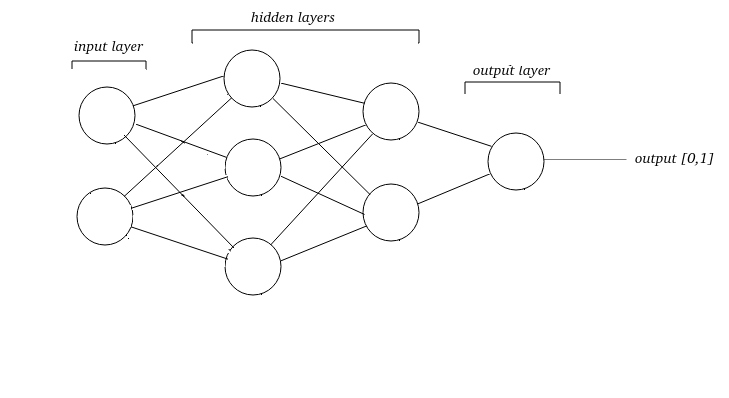
\includegraphics[scale = 0.55]{images/MLPClass}
 \caption {\textit{Esempio di MLPClassier generato da un individuo con cromosoma [3,2]}}
 \label{MLP}
\end{figure}

Infine si sfrutta il \textit{test set} per attribuire un \textit{fitness}, o \textit{score}, all'individuo.
Ciò viene fatto utilizzando due metri di valutazione differenti, valutati in parallelo: 

\paragraph{\textit{Accuracy score}} questo metodo è il più semplice e diretto: attribuisce un fitness pari alla percentuale di risposte corrette della rete. Il problema di questo procedimento è che equipara una risposta di $0.51$ ad $1$ ed una di $0.49$ a $0$ nonostante in entrambe le risposte l'incertezza sia alta.
L'\textit{accuracy score} viene massimizzato nell'algoritmo.

\paragraph{\textit{Logarithmic loss function}} o \textit{log loss}, è una misura di quanta incertezza pone la rete nelle sue risposte. Dalla documentazione di \textit{scikit learn} la \textit{log loss} è definita come "\textit{the negative log-likehood of the true labels given a probabilistic classifier's prediction}" o:  

\begin{equation}
 -log P(\frac{y_{t}}{y_{p}}) = -(y_{t} log(y_{p}) + (1 - y_{t}) log(1 - y_{p}))
\end{equation}
Dove $y_{t}$ è la classe dell'oggetto (o $0$ o $1$ ), mentre $y_{p}$ è la probabilità stimata che l'oggetto sia di quella classe.

Una caratteristica della log loss è la presenza di un limite superiore (che quantifica quanto incerta può essere al massimo una rete) che è possibile stimare estraendo a caso dei numeri tra 0 e 1 (simulando praticamente un addestramento nullo) e misurando lo score risultante: si ottiene cosi una stima pari a  $-ln(0.5) \approx 0.7$.

Non è stata attribuita nessuna forma di penalità alla profondità delle reti o, più in generale, a quanti collegamenti essa forma, che potrebbero quindi diventare sempre più grandi e computazionalmente pesanti da gestire, ma verrà studiato in seguito come si comportano queste grandezze (numero di collegamenti e lunghezza). 

Ogni MLP viene addestrato e valutato su due sezioni diverse del dataset: \textit{train set} e \textit{test set}.
Entrambe rappresentano una frazione dell'intero dataset scelta casualmente, in particolare sono rispettivamente l'80\textdiscount e il \textdiscount del dataset.
Nel \textit{train set} l'MLP viene addestrato mentre nel \textit{test set} viene valutato e gli viene attribuito uno score sulla base di questo risultato. 
Questa separazione serve per evitare l'\textit{overfitting} delle reti e in seguito verrà discusso come l'unico tipo di penalità che una rete molto complessa possa subire.

\section{Datasets}

I set di dati sono artificiali e forniti da \textit{scikit learn}. 
Sono stati usati per le prove 3 tipi di dataset:

\paragraph{moons} I punti rossi e blu vengono generati a forma di "semicerchi", come mostrato in figura \ref{moons} 

\begin{figure}[H]
 \centering
 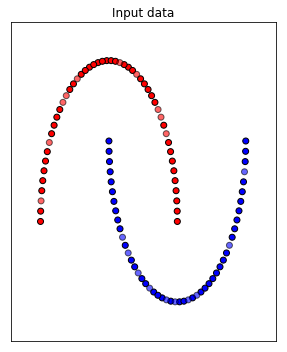
\includegraphics[scale = 0.5]{images/moons_nonoise}
 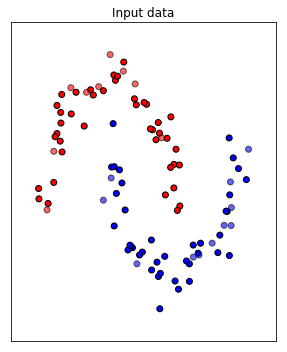
\includegraphics[scale = 0.5]{images/moons_noise}
 \caption{\textit{Nell'immagine sono messe a confronto due versioni del dataset moons: a sinistra priva di noise e a destra con noise = 0.1}}
 \label{moons}
\end{figure}

In questo caso i due gruppi hanno deviazioni standard simili ma medie diverse.

\paragraph{circles} I punti vengono generati a forma di cerchi concentrici, è possibile fornire diversi gradi di separazione ai due cerchi attraverso il parametro \textit{factor}. Il dataset è mostrato in figura \ref{circles}

\begin{figure}[H]
 \centering
 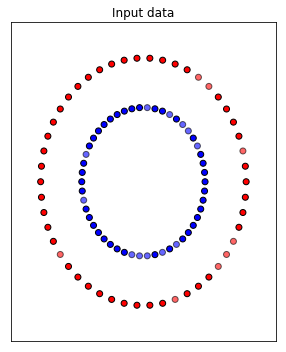
\includegraphics[scale = 0.5]{images/circles_nonoise}
 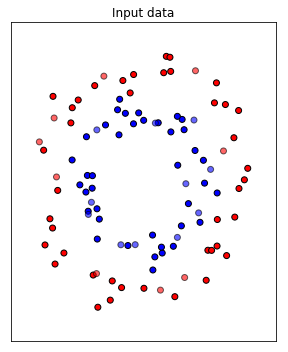
\includegraphics[scale = 0.5]{images/circles_noise}
 \caption{\textit{Nell'immagine a confronto due versioni del dataset circles: a sinistra senza noise e a destra con noise = 0.1. Entrambe con lo stesso fattore tra i cerchi}}
 \label{circles}
\end{figure}

Qui i due gruppi hanno medie simili ma deviazioni standard diverse, inoltre non sono separabili linearmente se non attraverso una trasformazione in coordinate polari.

\paragraph{circles+} È un dataset personalizzato creato dall'unione di due \textit{circles}, come mostrato in figura \ref{circles+}

\begin{figure}[H]
 \centering
 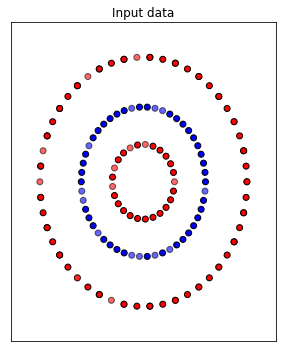
\includegraphics[scale = 0.5]{images/circles+_nonoise}
 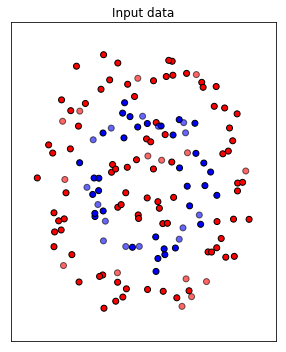
\includegraphics[scale = 0.5]{images/circles+_noise}
 \caption{\textit {Nell'immagine a confronto due versioni del dataset circles+: a sinistra con noise = 0 e a destra con noise = 0.1 }}
 \label{circles+}
\end{figure}

Questo dataset non permette nemmeno un tipo di separazione simile a quello descritto nel paragrafo precedente.

Per tutti i datasets è possibile attribuire un \textit{noise} in modo che sia più difficile separare le due classi di punti.
Nel corso delle prove sono state valutate le prestazioni dell'algoritmo su tutti i datasets.
Sono stati appositamente evitati dataset lineramente separabili.

I dataset sono generati a partire dalle due funzioni \textit{make moons} e \textit{make circles} di \textit{scikit learn}.


\section{Struttura dell'algoritmo }

Per chiarezza viene riportata la struttura dell'algoritmo, che ne mostra i vari passaggi:

\begin{enumerate}
 \item creazione della prima generazione.
 \item generazione del dataset, separazione di questo in \textit{train set} e \textit{test set}, valutazione del \textit{fitness} e ordinamento della popolazione.
 \item finché l'individuo con il \textit{best fitness} non rimane lo stesso per 5 generazioni consecutive:
 \begin{enumerate}
  \item[a.] separazione del dataset in \textit{train set} e \textit{test set} con \textit{random state} differenti ad ogni ciclo.
  \item[b.] Finchè la nuova generazione non è riempita ripetere:
  \begin{enumerate}
   \item [-] Selezione del primo e secondo genitore.
   \item [-] Crossover e creazione dei figli.
   \item [-] Mutazione dei figli.
  \end{enumerate}
  \item [c.] Valutazione del fitness e ordinamento della nuova generazione
  \item [d.] Risultati del migliore individuo sul dataset scelto.
 \end{enumerate}
 \item Termine dell'algoritmo nel caso il membro della popolazione con miglior fitness rimanga lo stesso per 5 generazioni di fila.
\end{enumerate}

Ogni iterazione di questo processo viene chiamata \textit{run}

\newpage

\section{Analisi Dati}

L'analisi dei dati può essere suddivisa in due parti: nella prima lo studio si concentra sulla capacità dell'algoritmo di separare le due classi di punti in ogni set di dati e con ognuna delle modalità presentate in precedenza, mostrando in ogni caso l'evoluzione qualitativa della migliore rete per ogni generazione.

Nella seconda parte ci si concentra invece su un'analisi quantitativa di alcune grandezze che caratterizzano la rete neurale: il numero di \textit{hidden layer}, la grandezza del layer con minore numero di neuroni e il numero di collegamenti che produce.
Il numero di \textit{hidden layer} altro non è che la sua lunghezza (o profondità), il numero di collegamenti (o link) dipende invece dal numero di neuroni totali infatti, in una rete \textit{fully connected}, è definito come:

\begin{equation}
 L = \sum_{i = 1}^{N-1} n_{i}n_{i+1}
\end{equation}

dove $n_{i}$ è il numero di neuroni dell'$i$-esimo layer e $N$ è il numero totale di layer.
Quindi prendendo ad esempio la rete [2,4,3] questa avrà $2\cdot2 + 2\cdot4 + 4\cdot3 + 3\cdot1 = 27$ link, contando anche i layer di input e di output.

Queste grandezze sono prese come misura della complessità della rete.

Ognuna di queste è stata studiata in funzione del \textit{noise} del dataset come misura di quanto questo risulti separabile: un dataset più rumoroso risulta inevitabilmente più difficile da classificare, sopratutto nel momento in cui punti blu e rossi siano molto vicini.
In questo secondo caso vengono effettuate numerose simulazioni e da ognuna vengono estratti i dati citati sopra dalla rete di convergenza.
Dopodichè viene mostrata la media punto per punto in funzione del noise ed in funzione dello score ottenuto a quel livello di noise.

\chapter{Risultati}

In questo capitolo verranno presentati i dati ottenuti confrontando le  metodologie discusse nel capitolo precedente.

\section{Classificazione dei dataset}

La prima parte dei risultati si concentra nell'analisi delle prestazioni dell'algoritmo nell'evolvere una popolazione di reti in grado di separare due classi di punti nei tre dataset presentati in precedenza. Verranno analizzate le prestazioni dei due algoritmi di selezione insieme ai due tipi di funzione di fitness.

\subsection{Moons Dataset}

Il primo dataset su cui è stato testato l'algoritmo è \textit{moons}, nelle immagini successive vengono riportati alcuni esempi di run effettute, differenziando \textit{Accuracy score} e \textit{log loss}, cioè i due diversi tipi di \textit{fitness function}, e i due algoritmi di selezione, che sono \textit{random mate} e \textit{all sons}.

In figura \ref{moons1} viene mostrata una run d'esempio utilizzando l'accuracy score:

\begin{figure}[H]
 \centering
 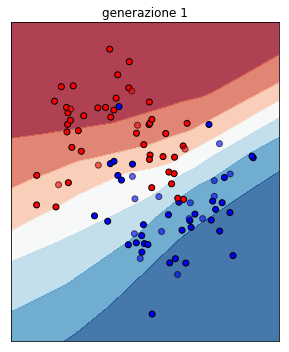
\includegraphics[scale = 0.5]{images/moons-rnd-acc./1}
 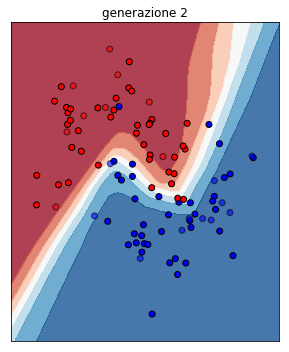
\includegraphics[scale = 0.5]{images/moons-rnd-acc./2}
 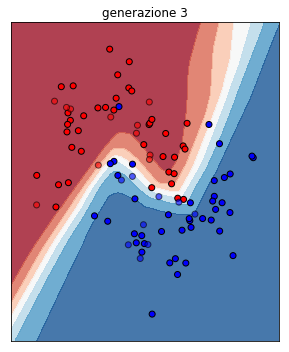
\includegraphics[scale = 0.5]{images/moons-rnd-acc./3}
 %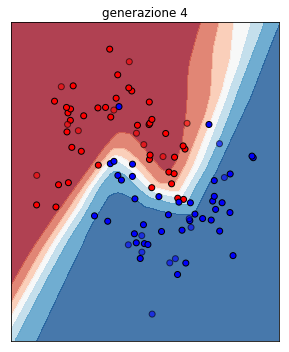
\includegraphics[scale = 0.4]{images/moons-rnd-acc./4}
 \caption{\textit{L'immagine mostra una run tipica usando l'accuracy score e la random mate selection e noise = 0.25}}
 \label{moons1}
\end{figure}

Nella figura \ref{moons1} viene mostrata una run rappresentativa effettuata utilizzando come algoritmo di Selezione \textit{random mate}: da notare come queste classificazioni raggiungano uno score molto alto (generalmente 100\textdiscount) nonostante la "sicurezza" della rete non sia molto alta nella classicazione di alcuni punti, specialmente se questi si trovano vicini a punti della classe opposta.
Questo accade perché lo score della rete viene valutato come se questa restituisse una risposta binaria per ogni input (0/1 o rosso/blu) e ciò è indipendente dall'incertezza con la quale viene determinata la classe di un punto. 
Ciò significa che per l'\textit{accuracy score} se un risultato è 0.01 o 0.49 questo sarà sempre o corretto o sbagliato a seconda che il valore vero sia 0 o 1, nonostante il secondo risultato sia pieno di incertezza.  
La "sicurezza" della rete è rappresentata sui grafici dal colore: tanto più è intenso e tanto  più il \textit{Multi-layer perceptron} è sicuro della sua scelta.
Il colore viene quantificato dalla funzione \textit{predict proba} di \textit{scikit learn}, che restituisce la probabilità calcolata dalla rete che un punto sia rosso o blu.

Alcune generazioni (le ultime) vengono escluse dalle immagini perchè, come detto nel capitolo precedente, sono tutte uguali.

In figura \ref{best1} viene invece mostrato il grafico del fitness del miglior individuo in funzione della generazione:

\begin{figure}[H]
 \centering
 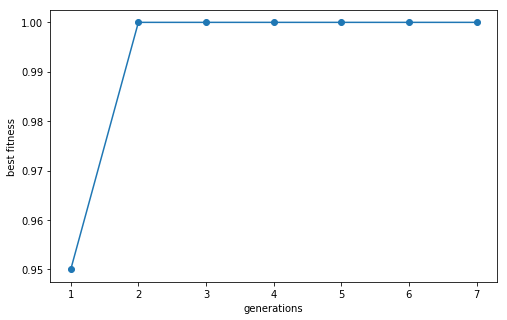
\includegraphics[scale = 0.5]{images/moons-rnd-acc./best}
 \caption{\textit{Best fitness di ogni generazione della popolazione con accuracy score e random mate}}
 \label{best1}
\end{figure}

Da notare come su questo dataset il raggiungimento di un individuo con fitness molto alto (di fatto insuperabile) sia molto veloce (in questo caso di una sola generazione), nonostante la separazione sembri molto incerta, come specificato sopra.

Risultati simili vengono raggiunti dal secondo algoritmo di selezione, mostrati in figura \ref{moons2}:

\begin{figure}[H]
 \centering
 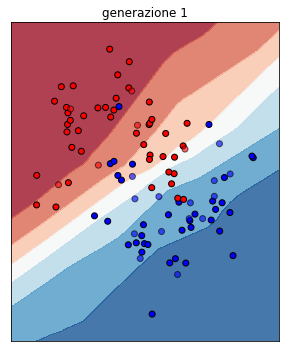
\includegraphics[scale = 0.5]{images/moons-sons-acc./1}
 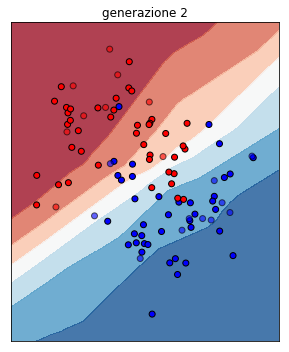
\includegraphics[scale = 0.5]{images/moons-sons-acc./2}
 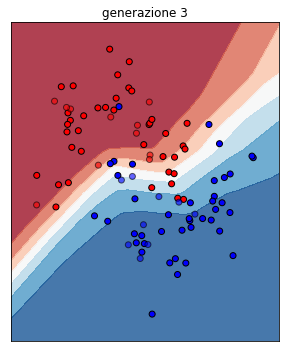
\includegraphics[scale = 0.5]{images/moons-sons-acc./3}
 %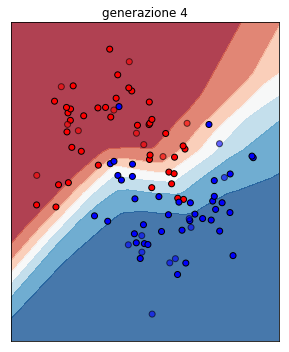
\includegraphics[scale = 0.35]{images/moons-sons-acc./4}
 \caption{\textit{In figura viene mostrata una run d'esempio utilizzando lo stesso noise e stessa funzione di fitness ma diverso algoritmo di selezione}}
 \label{moons2}
\end{figure}

Anche in questo l'evoluzione è rapida e il risultato finale incerto, nonostante l'ottimo risultato raggiunto dalle reti nell'\textit{accuracy test}. L'andamento del \textit{best fitness} è identico a quello precedente (figura \ref{best2}):

\begin{figure}[H]
 \centering
 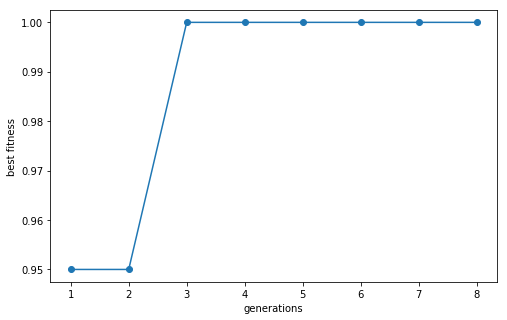
\includegraphics[scale = 0.5]{images/moons-sons-acc./best}
 \caption{\textit{In figura viene mostrato l'andamento del best fitness in funzione della generazione}}
 \label{best2}
\end{figure}

Data l'inefficienza sia computazionale sia in termini di performance, è stato deciso di abbandonare questo algoritmo di selezione per i prossimi datasets.


Significative differenze su questo dataset si hanno cambiando il tipo di funzione di fitness e passando alla \textit{logaritmic loss}, come mostrato in figura \ref{moons3}

\begin{figure}[H]
 \centering
 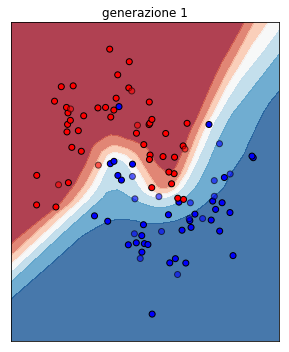
\includegraphics[scale = 0.37]{images/moons-rnd-log./1}
 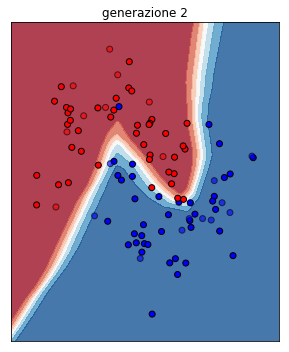
\includegraphics[scale = 0.37]{images/moons-rnd-log./2}
 \\
 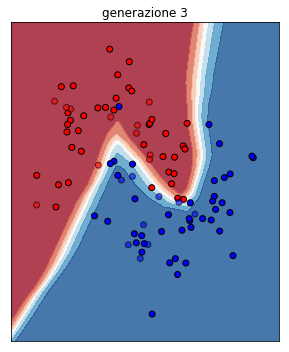
\includegraphics[scale = 0.37]{images/moons-rnd-log./3}
 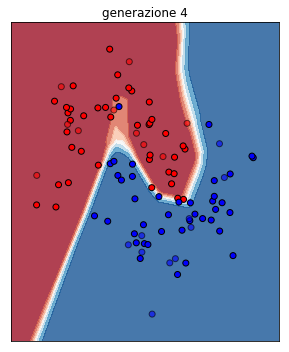
\includegraphics[scale = 0.37]{images/moons-rnd-log./4}
 \caption{\textit{Evoluzione di una rete neurale seguendo la logarithmic loss function sul dataset moons}}
 \label{moons3}
\end{figure}

\subsection{Circles Dataset}

Vengono presentati in forma parallela alla sezione precedente i risultati ottenuti dall'algoritmo nel dataset \textit{circles}, con noise = 0.2

\begin{figure}[H]
 \centering
 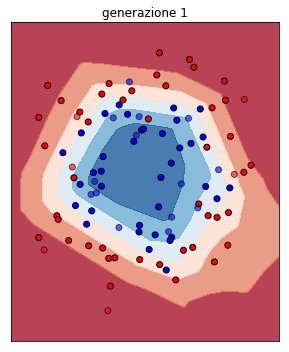
\includegraphics[scale = 0.5]{images/circles-rnd-acc/1}
 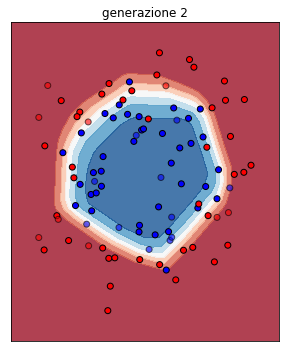
\includegraphics[scale = 0.5]{images/circles-rnd-acc/2}
 \\
 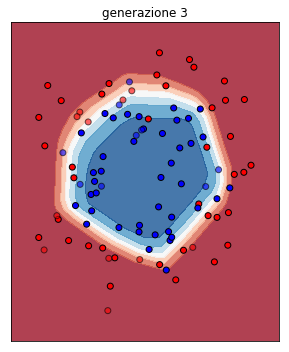
\includegraphics[scale = 0.5]{images/circles-rnd-acc/3}
 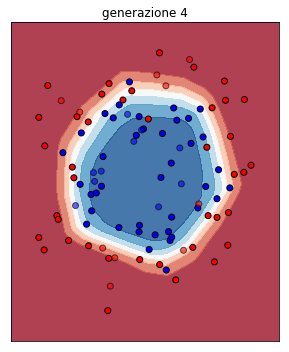
\includegraphics[scale = 0.5]{images/circles-rnd-acc/4}
 \caption{\textit{L'immagine mostra una run d'esempio nel dataset circles usando l'accuracy score}}
 \label{circles1}
\end{figure}

Anche in questo caso l'accuracy score mostra una convergenza dell'algoritmo molto rapida e approssimativa nella classificazione.

\begin{figure}[H]
 \centering
 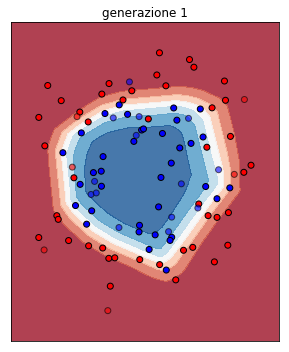
\includegraphics[scale = 0.5]{images/circle-rnd-log/1}
 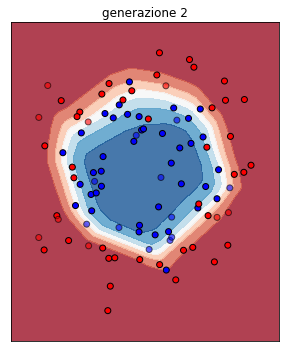
\includegraphics[scale = 0.5]{images/circle-rnd-log/2}
 \\
 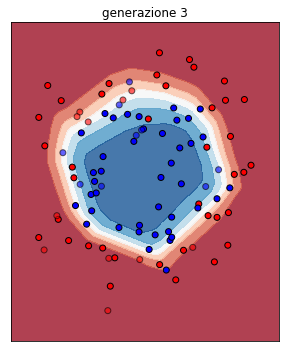
\includegraphics[scale = 0.5]{images/circle-rnd-log/3}
 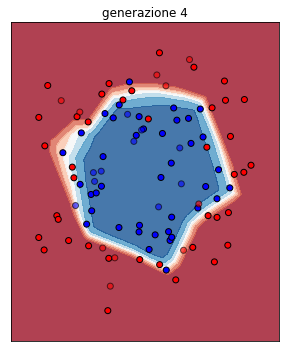
\includegraphics[scale = 0.5]{images/circle-rnd-log/4}
 \caption{\textit{L'immagine mostra una run d'esempio nel dataset circles usando la log loss}}
 \label{circles2}
\end{figure}

Come per il precedente dataset, questa funzione di fitness sembra riportare una classificazione più precisa, come mostrato in figura \ref{circles2}.

\newpage

\subsection{Circles+ Dataset}

I risultati più interessanti in termini di evoluzione della popolazione provengono dal dataset \textit{Circles+}, ideato come "stress test" per l'algoritmo. Nelle figure \ref{circles+1} e \ref{circles+2} vengono riportati i dati di classificazione.

In figura \ref{circles+1} è riportata una classificazione d'esempio utilizzando l'\textit{accuracy score functions}:

\begin{figure}[H]
 \centering
 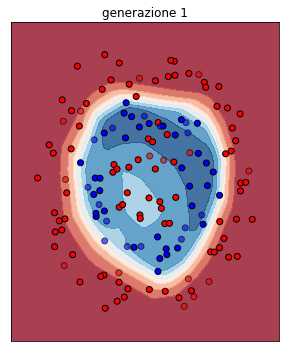
\includegraphics[scale = 0.35]{images/circle+-rnd-acc./1}
 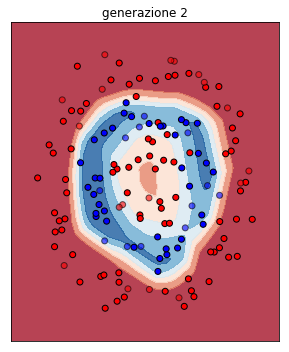
\includegraphics[scale = 0.35]{images/circle+-rnd-acc./2}
 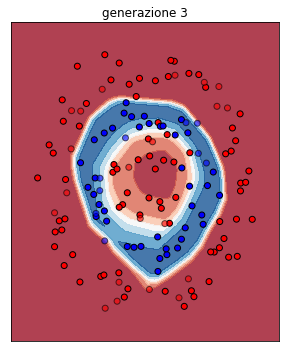
\includegraphics[scale = 0.35]{images/circle+-rnd-acc./3}
 \\
 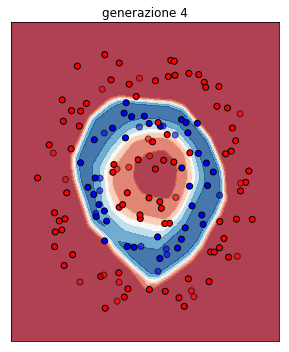
\includegraphics[scale = 0.35]{images/circle+-rnd-acc./4}
 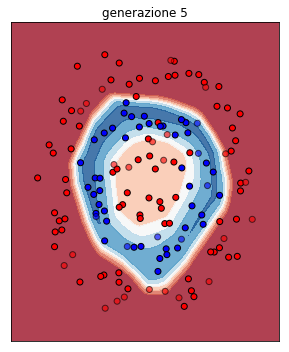
\includegraphics[scale = 0.35]{images/circle+-rnd-acc./5}
 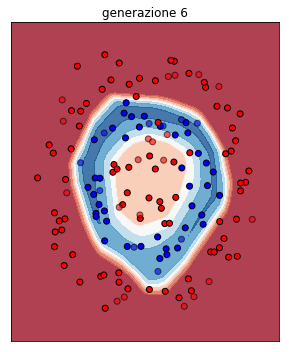
\includegraphics[scale = 0.35]{images/circle+-rnd-acc./6}
 \\
 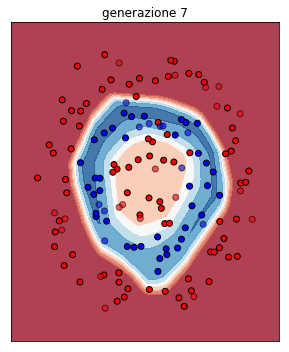
\includegraphics[scale = 0.35]{images/circle+-rnd-acc./7}
 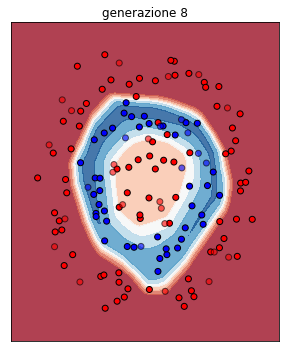
\includegraphics[scale = 0.35]{images/circle+-rnd-acc./8}
 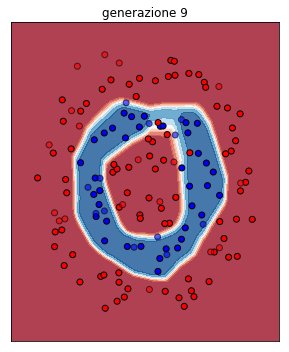
\includegraphics[scale = 0.35]{images/circle+-rnd-acc./9}
 \caption{\textit{L'immagine mostra una run d'esempio nel dataset circles+ usando l'accuracy score}}
 \label{circles+1}
\end{figure}

Infine viene mostrata una run d'esempio utilizzando la \textit{logarithmic loss function}.

\begin{figure}[H]
 \centering
 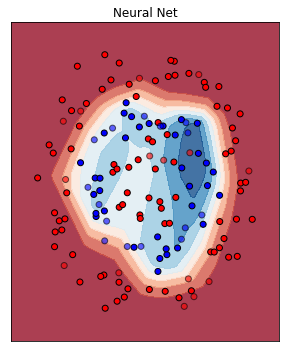
\includegraphics[scale = 0.37]{images/circle+-rnd-log./1}
 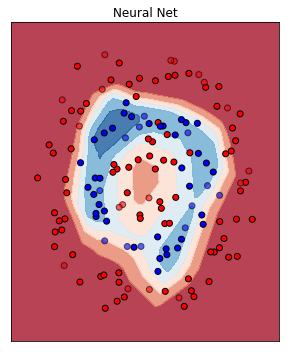
\includegraphics[scale = 0.37]{images/circle+-rnd-log./2}
 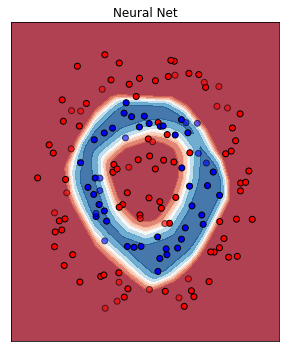
\includegraphics[scale = 0.37]{images/circle+-rnd-log./3}
 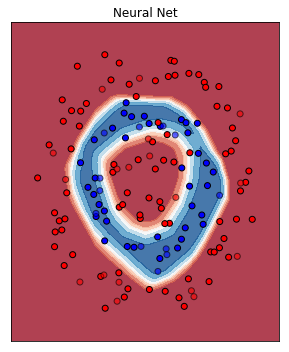
\includegraphics[scale = 0.37]{images/circle+-rnd-log./4}
 \\
 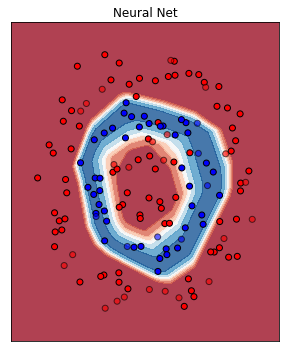
\includegraphics[scale = 0.37]{images/circle+-rnd-log./5}
 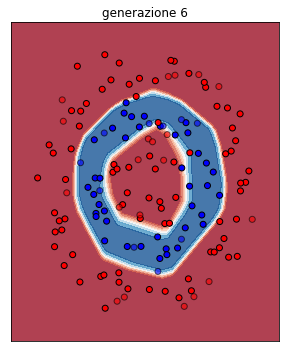
\includegraphics[scale = 0.37]{images/circle+-rnd-log./6}
 \includegraphics[scale = 0.37]{images/circle+-rnd-log./7}
 \includegraphics[scale = 0.37]{images/circle+-rnd-log./8}
 \\
 \includegraphics[scale = 0.37]{images/circle+-rnd-log./9}
 \includegraphics[scale = 0.37]{images/circle+-rnd-log./10}
 \includegraphics[scale = 0.37]{images/circle+-rnd-log./11}
 \caption{\textit{L'immagine mostra una run d'esempio nel dataset circles+ usando la log loss con noise = 0.1}}
 \label{circles+2}
\end{figure}

In questo caso la convergenza è molto simile nelle due funzioni di fitness.
In entrambe le simulazioni è possibile osservare un'evoluzione più lenta rispetto ai primi due dataset.
In particolare questa evoluzione inizia da una popolazione casuale che non riconosce (per nulla o in parte) il cerchio interno di punti di colore rosso ma avanzando nelle generazioni questo gruppo interno viene correttamente classificato. 
Dopodichè in entrambi i casi l'evoluzione porta ad un miglioramento della precisione della separazione fino alla convergenza, la quale risulta 

\newpage

\section{Complessità della rete} 

I parametri importanti da considerare nel valutare la complessità di una rete sono:

\begin{enumerate}
 \item[-] Collegamenti
 \item[-] Numero di neuroni del layer più piccolo
 \item[-] Numero di \textit{Hidden Layer}
\end{enumerate}

Questi ci danno una misura di quanta informazione può contenere e quanto è possibile comprimerla.
Nell'algoritmo genetico non è stata impostata alcuna penalità in relazione alla complessità della rete, l'obiettivo infatti non è stato quello di trovare la rete più performante in termini computazionali, quindi esiste la possibilità che non converga mai ad un risultato finale, costruendo reti sempre più profonde e precise nel separare i dati.
In realtà ciò non è osservato nei casi elencati fino ad ora, ossia quando le due classi non sono perfettamente separabili. 
Inoltre, come già accennato, per la funzione di fitness \textit{accuracy score} non può succedere perché prima o poi l'algoritmo convergerà ad una soluzione con score pari a $100$\textdiscount, di fatto insuperabile.

La situazione è diversa per la \textit{log loss} che invece ha un limite inferiore asintotico: nel senso che è idealmente impossibile trovare una rete perfetta di score nullo (nel seguito fitness molto bassi vengano trattati come 0, questo perché differenziare un $3\cdot10^{-5}$ da un $2\cdot10^{-5}$ in termini pratici è irrilevante: entrambe le reti sono state abbastanza precise da classificare ogni punto correttamente nonostante per l'algoritmo la seconda sia migliore).    
Per questo motivo è stato studiato il comportamento dell'algoritmo con questa funzione di fitness al variare della separabilità dei dati, quantificata dal rumore.

L'obiettivo è quindi quello di studiare l'andamento di questi parametri in funzione del \textit{noise} dei dataset.

\newpage

\subsection{Moons Dataset}

Iniziamo con il presentare i dati relativi all'andamento del fitness delle reti in funzione del noise introdotto nel dataset \textit{moons} in figura \ref{score_moons}.

\begin{figure}[H]
 \centering
 \includegraphics[scale = 0.7]{images/score_noise_moons.png}
 \caption{\textit{Nel grafico viene mostrato l'andamento dello score in funzione del noise del dataset. In evidenza alcuni punti interessanti dell'andamento}}
 \label{score_moons}
\end{figure}

Nel dataset \textit{moons} lo score non risulta sensibile ai cambiamenti del noise e rimane prossimo a 0 (per la \textit{logloss} uno score migliore rappresenta un fitness maggiore) fino a che la run raggiunge noise = 0.2: probabilmente questo è il valore in cui i punti non sono più perfettamente separabili.
Il grafico non sembra mostrare un andamento di saturazione per alti livelli di noise, ciò significa che nonostante le reti ancora riescono a distinguere alcuni punti rossi e blu.

Di seguito verranno mostrati gli andamenti delle grandezze scelte come rappresentative della complessità della rete.

\begin{figure}[H]
 \centering
 \includegraphics[scale = 0.6]{images/links_noise_moons}
 \includegraphics[scale = 0.6]{images/Links_Score_moons}
 \caption{\textit{A confronto gli andamenti del numero di collegamenti in funzione del noise ed in funzione dello score}}
 \label{linksmoons}
\end{figure}

In figura \ref{linksmoons} viene mostrato l'andamento dei collegamenti della rete in funzione del noise e del fitness.

Nel primo grafico si nota un andamento fortemente decrescente anche nel range di valori di noise in cui lo score del dataset è costante a 0. Aumentando ancora il noise l'andamento si stabilizza rimanendo comunque decrescente. Se per \textit{noise} prossimi allo zero la rete raggiunge un numero di collegamenti elevato (5000 collegamenti in media per noise = 0), questo crolla quando il noise raggiunge certi valori e continua a decrescere poi.

Nel secondo grafico si nota una rapida divergenza nel numero di links avvicinandosi a valori di score  prossimi a 0: se l'algoritmo riesce a classificare molto bene il dataset allora tende a cercare reti con un numero di collegamenti più elevato.

Nella figura successiva, la \ref{smallmoons}, verrà presentato l'andamento del numero di neuroni nel layer più piccolo della rete in funzione del noise e dello score.

\begin{figure}[H]
 \centering
 \includegraphics[scale = 0.5]{images/small_noise_moons}
 \includegraphics[scale = 0.5]{images/small_Score_moons}
 \caption{\textit{Nei due grafici sono mostrati gli andamenti del numero di neuroni nel layer più piccolo della rete in funzione del noise di moons e dello score}}
 \label{smallmoons}
\end{figure}

In questo dataset, il numero di neuroni del layer più piccolo della rete mostra un andamento costante sia in funzione del noise e sia in funzione dello score. 

\begin{figure}[H]
 \centering
 \includegraphics[scale = 0.5]{images/depth_noise_moons}
 \includegraphics[scale = 0.5]{images/depth_Score_moons}
 \caption{\textit{Studio dell'andamento del numero della profondità della rete in funzione del noise e dello score per il dataset moons. In evidenza i punti di noise che mostrano andamenti interessanti(rispettivamente 0.1,0.2 e 0.6)}}
 \label{noisemoons}
\end{figure}

Come per i link, anche in questo l'andamento della profondità in funzione del Noise è fortemente decrescente anche se sembra mostrare un accentuato plateau nel range di noise da 0.3 fino a noise = 0.6.
La lunghezza delle reti avvicinandosi a score molto bassi tende a divergere, proprio come il numero di collegamenti.

Vengono riportate di seguito in figura \ref{exnoisemoons} alcuni esempi di come si mostra un classificazione effettuta a diversi livelli di noise per \textit{moons}.
Le reti che hanno effetuato tali classificazione sono[17, 20, 24, 23, 24, 26, 20, 24, 23, 24, 26, 17, 9, 14, 6],[7, 12, 13, 24, 22], [24, 23, 13] e [6, 21]

\begin{figure}[H]
\centering
 \includegraphics[scale = 0.5]{images/moons-noise0,1}
 \includegraphics[scale = 0.5]{images/moons-noise0,3}
 \includegraphics[scale = 0.5]{images/moons-noise0,6}
 %\includegraphics[scale = 0.35]{images/moons-noise1}
 \caption{\textit{in figura viene mostrata una classificazione d'esempio su diversi livelli di noise, da sinistra : noise = 0.1,noise = 0.2 e noise = 0.6}}
 \label{exnoisemoons}
\end{figure}

In figura \ref{exnoisemoons} sono mostrati 3 momenti significativi del dataset: prima della presunta transizione, quando i punti sono ancora perfettamente separabili, durante la transizione a noise = 0.2 quando i punti iniziano a mischiarsi e a  non essere più separabili dalla rete e infine a noise = 0,6, ben oltre la transizione, quando i punti sono definitavemente impossibili da separare se non approssimativamente.

\newpage

\subsection{Circles Dataset}

Il secondo dataset analizzato è \textit{circles}, di seguito vengono mostrati i dati ottenuti:
In figura \ref{score_circles} viene mostrato l'andamento dello score in funzione del noise del dataset.

\begin{figure}[H]
 \centering
 \includegraphics[scale = 0.7]{images/score_noise_circles.png}
 \caption{\textit{Nel grafico viene mostrato l'andamento dello score in funzione del noise del dataset. In evidenza alcuni punti interessanti dell'andamento}}
 \label{score_circles}
\end{figure}

Notiamo che anche per \textit{circles} esiste una zona di classificazione perfetta in cui lo score sembra indipendente rispetto al noise al dataset.
Inoltre, a differenza di \textit{moons}, qui lo score sembra raggiungere un livello di saturazione, simbolo del fatto che raggiunto un certo noise, i punti blu e rossi sono impossibili da separare per la rete. 

Di seguito sono presentati i grafici delle tre grandezze che caratterizzano la complessità della rete per il dataset \textit{circles}:

\begin{figure}[H]
 \centering
 \includegraphics[scale = 0.5]{images/links_noise_circles}
 \includegraphics[scale = 0.5]{images/Links_Score_circles}
 \caption{\textit{Andamento dei collegamenti delle reti in funzione di noise e score}}
 \label{link-circles}
\end{figure}

In figura \ref{link-circles} vengono mostrati gli andamenti dei link in funzione del rumore del dataset ed in funzione dello score ottenuto dalla rete di convergenza.
Vediamo che il numero di link tende a decrescere rapidamente nonostante nel range di noise [0;0.1] lo score della classificaziione sia costante. A differenza che nel caso di \textit{moons} il numero di collegamenti sembra convergere.
Si nota un plateau intorno a valori di noise = 0.2.

Nel secondo grafico invece osserviamo ancora una volta una divergenza per score bassi e quindi buone classificazioni, mentre un andamento molto rumoroso intorno ad un noise = 0.6

In figura \ref{small-circles} vengono mostrati gli andamenti relativi al numero di neuroni con layer più piccolo nella rete: 

\begin{figure}[H]
 \centering
 \includegraphics[scale = 0.5]{images/small_noise_circles}
 \includegraphics[scale = 0.5]{images/small_Score_circles}
 \caption{\textit{Andamento dello smaller layer in funzione di noise e score.}}
 \label{small-circles}
\end{figure}

Notiamo un andamento decrescente nel numero di neuroni del layer più piccolo a differenza di quanto osservato per il precedente dataset.
Ancora una volta la parte per score più alti e classificazioni peggiori risulta molto rumorosa per questo dataset.

In figura \ref{depth_circles} vengono riportati i dati ottenuti sulla profondità della rete in funzione di noise e score.

\begin{figure}[H]
 \centering
 \includegraphics[scale = 0.5]{images/depth_noise_circles}
 \includegraphics[scale = 0.5]{images/depth_Score_circles}
 \caption {\textit{In figura viene mostrato l'andamento della profondità delle reti in funzione del noise e dello score}}
 \label{depth_circles}
\end{figure}

Gli andamenti appaiono simili a quelli osservati per i link nello stesso dataset.

In figura \ref{exnoisecircles} sono raffigurati 4 esempi di classificazione di \textit{circles} a livelli diversi di noise. Le reti che hanno compiuto queste classificazioni sono rispettivamente [16, 24, 24, 20, 24, 23, 24, 24, 23, 22, 24, 14, 24, 16, 14, 20], [19, 22, 19, 5, 14] e [18, 24, 18, 10]:

\begin{figure}[H]
 \centering
 \includegraphics[scale = 0.4]{images/circles-noise0,1.png}
 \includegraphics[scale = 0.4]{images/circles-noise0,2.png}
 \includegraphics[scale = 0.4]{images/circles-noise0,6.png}
 %\includegraphics[scale = 0.35]{images/circles-noise1.png}
 \caption{\textit{in figura viene mostrata una classificazione d'esempio su diversi livelli di noise, da sinistra : noise = 0,1 quando ancora i punti sono separabili, noise = 0.2 e noise = 0.6 quando i punti sono pressochè indistinguibili dalla rete}}
 \label{exnoisecircles}
\end{figure}

I tre esempi mostrano bene il cambiamento che compie il dataset durante la prova.
Notiamo inoltre come l'algoritmo dopo un certo noise non riesca più a classificare efficacemente il dataset.

\subsection{Circles+ Dataset}

Terzo ed ultimo dataset presentato è \textit{circles+} che combina due dataset \textit{circles}.
Nel grafico in figura \ref{score-circles+} viene mostrato l'andamento del fitness della rete di convergenza in funzione del noise del dataset.

\begin{figure}[H]
 \centering
 \includegraphics[scale = 0.6]{images/score_noise_circles+}
 \caption{\textit{Andamento dello score in funzione del noise per il dataset circles+}}
 \label{score-circles+}
\end{figure}

Anche in questo caso si nota un range di noise per cui lo score della classificazione rimane costante a 0(più ristretto di quelli precedenti) e infine si nota un valore di saturazione per lo score.

In figura \ref{links-score-circle+} sono comparati gli andamenti dei link in funzione di noise e score:

\begin{figure}[H]
 \centering
 \includegraphics[scale = 0.5]{images/links_noise_circles+}
 \includegraphics[scale = 0.5]{images/Links_Score_circles+}
 \caption{\textit{Andamento dei links in funzione del noise del dataset e dello score ottenuto  }}
 \label{links-score-circle+}
\end{figure}

L'andamento del grafico dei links in funzione del noise è simile a quelli precedenti ma presenta uno \textit{spike} intorno al valore di noise =  0.2. Come per circle, sembra convergere ad un valore stabile.

\begin{figure}[H]
 \centering
 \includegraphics[scale = 0.5]{images/small_noise_circles+}
 \includegraphics[scale = 0.5]{images/small_Score_circles+}
 \caption{\textit{Andamento del numero di neuroni nel layer più piccolo in funzione del noise e dello score ottenuto}}
 \label{small-score-circle+}
\end{figure}

Come per il dataset \textit{circle} anche qui, osserviamo che il numero di neuroni nel layer minore diminusce all'aumentare del noise.

\begin{figure}[H]
 \centering
 \includegraphics[scale = 0.5]{images/depth_noise_circles+}
 \includegraphics[scale = 0.5]{images/depth_Score_circles+}
 \caption{\textit{Andamento della profondità in funzione del noise e dello score ottenuto }}
 \label{depth-score-circle+}
\end{figure}

Anche in questo caso, l'andamento della lunghezza in funzione del noise è molto simile all'andamento del numero di links.

In figura \ref{exnoisecircles+} vengono mostrati degli esempi di classificazione con diversi valori di noise.
Le reti alle quali l'algoritmo converge in questi casi sono rispettivamente: [24, 21, 20, 21, 20, 21, 4, 14, 21, 24, 6, 21], [22, 24, 24, 12] e []

\begin{figure}[H]
 \centering
 \includegraphics[scale = 0.4]{images/circles+-noise0,1.png}
 \includegraphics[scale = 0.4]{images/circles+-noise0,2.png}
 \includegraphics[scale = 0.4]{images/circles+-noise0,4.png}
 \caption{\textit{In figura viene mostrata una classificazione d'esempio su diversi livelli di noise, da sinistra : noise = 0,noise = 0.2 e noise = 0.6 }}
 \label{exnoisecircles+}
\end{figure}

Nel caso di \textit{circles+} si raggiunge in fretta un livello di noise tale da rendere impossibile all'algoritmo una classificazione anche approssimativa del dataset, tuttavia è ancora possibile ottenre una classificazione accurata per noise = 0.1
È facile immaginare che le classificazioni per noise > 0,6 non siano molto diverse da quella mostrata.

\chapter{Conclusioni}

In questo capitolo verranno discussi i principali risultati presentati nel capitolo precedente.
La separazione compiuta dall'algoritmo sui dataset composti da due classi di punti sembra essere buona sotto una certa soglia di rumore e ciò vale sia per l'\textit{accuracy score} sia per la \textit{logarithmic loss}, nonostante esistano delle nette differenze tra le due in capacità di classificazione, almeno per quanto osservato nei dataset \textit{circles} e \textit{moons}, nei quali la seconda risulta più precisa e meno approssimativa. 

Nel terzo dataset invece il comportamento sembra simile anche se, ancora una volta, la \textit{log loss} raggiunge un risultato più preciso se si considerano le zone di bordo tra punti rossi e blu. 
In generale, possiamo dire che per quanto riguarda questi semplici casi di classificazione di punti l'algoritmo riesce a trovare un individuo in grado di compiere una separazione più o meno netta (ciò dipende dal noise) nonostante lo spazio di ricerca sia molto vasto, ottenendo risultati migliori se invece di considerare la semplice risposta binaria della rete (blu/rosso) si considera la sicurezza con la quale la rete attribuisce tale risposta e si cerca di massimizzare tale certezza.

Naturalmente ciò non significa che l'MLP restituito dalla convergenza dell'algoritmo sia il migliore in termini di classificazione o in termini di costo computazionale, sia per il suo addestramento sia nel calcolare la sua risposta, che in caso di problemi complessi rappresenta sicuramente un problema. 

Per questo si è voluto analizzare anche la complessità della rete, quantificandola in tre parametri: Link, Numero di hidden layer (profondità o lunghezza) e numero di neuroni nel layer più piccolo.
Ricordando che non esiste nell'algoritmo genetico nessuna forma di penalità per reti troppo "grandi", sembra scontato affermare che in qualsiasi caso l'algoritmo tenderà a preferire un numero molto grande di hidden layer aumentandolo di generazione in generazione dato che in generale reti di questo tipo dovrebbe avere performance di classificazione migliore.
In realtà ciò accade solo nel caso di rumore molto basso o nullo: diminuendolo infatti in tutti e tre i dataset la lunghezza e il numero di link della rete crescono molto rapidamente, il che sembra rappresentare un comportamento totalmente anti-intuitivo. 

In altre parole la complessità della rete aumenta al diminuire della complessità del dataset: questa caratteristica potrebbe essere dovuta ad una sorta di penalizzazione interna all'addestramento degli MLP.
Infatti, la separazione tra \textit{train set} e \textit{test set} fa in modo che le reti che ottengono alti score sul primo (\textit{overfitting}) vengano in seguito penalizzate sul secondo.

Questo si vede su noise elevati ed in tutti e tre i casi sembra esistere un valore di soglia oltre il quale il fitness degli individui peggiora enormemente fino a raggiungere un valore stabile per i dataset \textit{circles}(intorno a 0.6) e \textit{circles+} (compreso tra 0.5 e 0.6), mentre per \textit{moons} questo non si osserva, molto probabilmente perché la rete è ancora in grado di distinguere due gruppi di punti.

Andando ad analizzare più in dettaglio i dataset:

\paragraph{\textit{moons :}} i dati confermano l'andamento generale descritto sopra a parte per il numero di link nel layer minore, che invece in questo caso rimane costante: ciò che ci dice che la minima compressione dell'informazione non dipende da quando sia rumoroso il dataset ne dallo score ottenuto dalla rete.
Confrontando il grafico dello score con quelli dei links osserviamo che mentre il primo rimane costante a 0, il secondo è quasi dimezzato, cosi come la profondità della rete. 
\paragraph{\textit{circles :}} il valore sul quale si stabilizza lo score è molto alto rispetto al punto che \textit{moons} raggiunge, probabilmente qui i punti sono completamente mischiati e non vi è traccia di qualche dato che la rete possa ricavare per riconoscerli. Ciò probabilmente è lo stesso motivo per cui gli andamenti di lunghezza delle reti e dei link si stabilizzano. Si osserva un andamento interessante attorno a noise = 0.2 , come un plateau, forse dovuto ad una regolarità nei dataset.
\paragraph{\textit{circles+ :}} gli andamenti sono simili a quelli di \textit{circles} anche se qui il valore di score stabile è leggermente più basso, anche se è più stretto il range di valori al quale il fitness rimane nullo: ciò è dovuto alle irregolarità di questo dataset che anche in condizioni di noise basso risulta più difficile da classificare per l'algoritmo.

In tutti i casi viene osservata quella che sembra essere una transizione di fase nella rete neurale dovuta alla rumorosità dei dati con cui ha a che fare.

Possibili sviluppi per l'algoritmo potrebbero essere l'introduzione di una penalità che scali in funzione della complessità della rete, in modo da evidenziare le differenze di comportamento tra le due versioni, sopratutto verificare se il comportamento della rete rimanga dipendente dalla rumorosità dei dati.
La limitazione a dati artificiali andrebbe superata in favore di dati reali su cui testarne il funzionamento.
Inoltre sarebbe interessante applicare questi metodi alle reti a convoluzione, un particolare tipo di reti neurali ispirate alla corteccia visiva animale, che sono una variazione del MLP e hanno diverse applicazioni nel riconoscimento di immagini e video.

\listoffigures


\nocite{*}
\addcontentsline{toc}{chapter}{Bibliografia}
\bibliographystyle{unsrt}
\bibliography{Bibliografia.bib}


\end{document}




